\documentclass{beamer}
\usetheme{ConnectivityLab}
\usepackage{times}
\usepackage{graphicx}
\usepackage{verbatim}
\usepackage{outlines}
\usepackage{fancyhdr}
\usepackage{subfigure}
\usepackage{cancel}
\usepackage{bibentry}
\usepackage{varwidth}
\usepackage{etoolbox}
\usepackage{epstopdf}
%%%%%%%%%%%%%%%%%%%%%%%%%%%%%%%%%%%%%%%%%%%%%%%%%%%%%%
%%%%%%%%%%%%%%%%%%%%%%%%%%%%%%%%%%%%%%%%%%%%%%%%%%%%%%

\title {
    Progress report
}
\author {
    Yin-Hong, Hsu
}
\date {
    03 23, 2017
}

%%%%%%%%%%%%%%%%%%%%%%%%%%%%%%%%%%%%%%%%%%%%%%%%%%%%%%
%%%%%%%%%%%%%%%%%%%%%%%%%%%%%%%%%%%%%%%%%%%%%%%%%%%%%%

\begin{document}
\begin{frame}
    \titlepage
\end{frame}

%%%%%%%%%%%%%%%%%%%%%%%%%%%%%%%%%%%%%%%%%%%%%%%%%%%%%%
%%%%%%%%%%%%%%%%%%%%%%%%%%%%%%%%%%%%%%%%%%%%%%%%%%%%%%

\begin{frame}{Outline}
    \tableofcontentsgather
    \tableofcontents
\end{frame}

%%%%%%%%%%%%%%%%%%%%%%%%%%%%%%%%%%%%%%%%%%%%%%%%%%%%%%
%%%%%%%%%%%%%%%%%%%%%%%%%%%%%%%%%%%%%%%%%%%%%%%%%%%%%%
\section{Extended Access Barring}

\begin{frame}{Briefly introduce EAB \cite{6489075}}
    \begin{itemize}
        \item {The device is divided into two types}
        \begin{itemize}    
            \item[-]{delay sensitive}
            \item[-]{delay tolerant}
        \end{itemize}
        \item {EAB is used for device which be delay-tolerant}
    \end{itemize}
\end{frame}

\begin{frame}{Briefly introduce EAB \cite{spec}}
    \begin{itemize}
        \item {There is 10 AC level for devices (0...9)}
        \item {In SIB14, there is a bitmap called barringBitmap, if the corresponding bit is 1, then the device will be barred}
        \item {It's not evolved from ACB}
    \end{itemize}
\end{frame}

\section{Process of Access Barring in NB-IOT}

\begin{frame}{NB-IoT v.s. LTE (different)}
    \begin{itemize}
        \item {NB-IoT adopt EAB as the based of access barring mechanism}
        \item {It's similar to access barring check of NB-IoT and EAB check, but NB-Iot has more If Else for there spec}
        \begin{itemize}    
            \item[-]{AC level 11...15}
            \item[-]{exception Data}
        \end{itemize}
    \end{itemize}
\end{frame}

\begin{frame} {access barring check for NB-IoT \cite{spec}}  
    \begin{figure}[t]
    \centering
    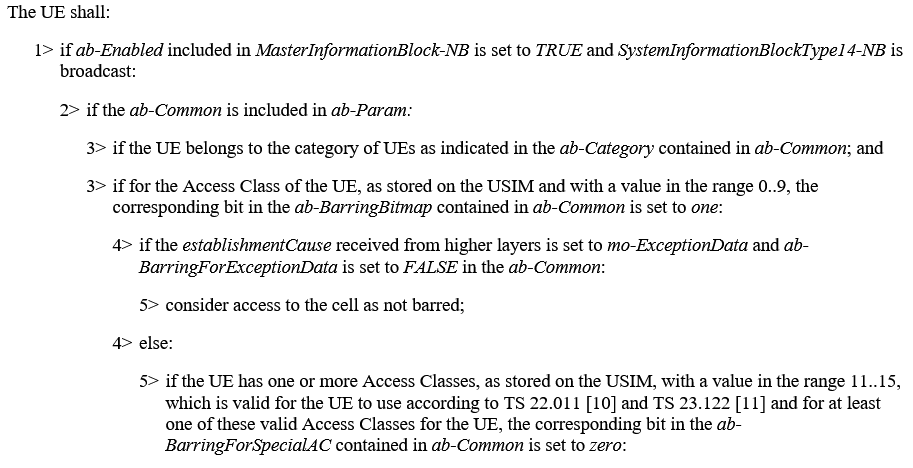
\includegraphics[width=1\textwidth]{figures/ab.png}
    \setbeamerfont{caption}{size=\tiny}
    \end{figure}
\end{frame}



%%%%%%%%%%%%%%%%%%%%%%%%%%%%%%%%%%%%%%%%%%%%%%%%%%%%%%
\section{References}
\calcreferencespagetotal % Calc your References Page total number
\begin{frame}[allowframebreaks]{References}
    \fontsize{9pt}{13}\selectfont
    \bibliographystyle{IEEEtran}
    \bibliography{IEEEabrv,Citation}
\end{frame}

%%%%%%%%%%%%%%%%%%%%%%%%%%%%%%%%%%%%%%%%%%%%%%%%%%%%%%
\section{}

\begin{frame}
    \centering
    \Large{Thanks for Your Attentions}
\end{frame}

\end{document}
